\documentclass[10pt,handout,usepdftitle=false,envcountsect]{beamer}

\usepackage[utf8]{inputenc}
\usepackage{listings}
\usepackage[francais]{babel}
\usepackage[T1]{fontenc}
\usepackage{tikz}
\usepackage{tikzscale}
\usepackage{tikz-uml}
\usepackage{scalefnt}
\usepackage{calc}
\usepackage{verbatim}
\usepackage{pgf-pie}
\usetheme{Singapore}
\usecolortheme{orchid}
\useinnertheme{rectangles}
\useoutertheme{smoothbars}


% Title Page
\title{Gestion de performances de courreurs}
\author{Quentin Le Guennec \newline http://github.com/AureoleMoka/gpc.git}
\institute{Lycée Pierre Méchain Laon}
\date{\today}

\begin{document}
\section{Présentation}

\begin{frame}
\centering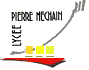
\includegraphics[scale=1]{pierre-mechain.png}
\maketitle
\end{frame}

\AtBeginSection[] {
    \begin{frame}{Sommaire}
        \tableofcontents[currentsection]
    \end{frame}
}
\subsection{Sommaire}
\frametitle{Sommaire}
\begin{frame}
\tableofcontents
\end{frame}

\subsection{Introduction}
\begin{frame}
\frametitle{Objectif du système}
\begin{block}{Objectifs}
\begin{itemize}
\item Gérer le déroulement d'une course automatiquement
\item Enregistrer les performances des courreurs
\item Présenter sur un support de son choix les performances d'un courreur
\end{itemize}
\end{block}
\end{frame}

\begin{frame}
\frametitle{Naming utilisé}
\begin{block}{Naming}
\begin{description}
\item[dbDial] Classe qui gère les dialogues avec la base de données
    \newline
\item[CodeReader] Lecteur de code barre pour idenfier un adhérent grâce à sa carte.
    \newline
\item[RFIDReader] Lecteur de badges par RFID pour attribuer à un courreur un ID
    \newline
\item[Portique] Lecteur de badges par RFID qui permet de notifier le passage d'un courreur
    \newline
\item[Michel] Désigne un participant, Adhérent ou non
\end{description}
\end{block}
\end{frame}

\begin{frame}
\frametitle{Prérequis}

\begin{block}{Software nécessaire}

\begin{description}
\item[Un browser] \hfill \\Pour afficher les performances
\item[Un serveur de base de données] \hfill \\Pour stocker les informations des adhérents
\item[Le client] \hfill \\Actuellement développé en C\#
\end{description}
\end{block}

\begin{block}{Hardware nécessaire}

\begin{description}
\item[Deux lecteur RFID] \hfill \\Un pour attribuer un badge à un participant et un portique RFID
\item[Un lecteur de code barre] \hfill \\Pour identifier les adhérents grâce à leur carte
\end{description}
\end{block}

\end{frame}

\subsection{Travail effectué}
\begin{frame}

\frametitle{Participants au projet}
    \begin{block}{Quentin Le Guennnec}
        site web et de la base de données, aide générale
        \newline\emph{Classes} CodeReader, dbDial
    \end{block}
    \begin{block}{Bastien Kopka} 
        design du site web, analyse des documentations
        \newline\emph{Classes} Portique, RFIDReader
    \end{block}
    \begin{block}{Léo David} 
        analyse des documentations
        \newline\emph{Classes} Portique, RFIDReader
        \newline
    \end{block}
\end{frame}

\begin{frame}
\frametitle{Répartition du temps}
\begin{alertblock}{Temps}
\begin{tikzpicture}[scale=0.6]
        \pie{12/Analyse des documentations, 15/Développement, 16/Analyse UML, 30/BDD et Serveur web, 27/Analyse du matériel}
\end{tikzpicture}
\end{alertblock}
\centering\begin{exampleblock}{Au total:} 
Environ 70 heures
\end{exampleblock}
\end{frame}


\section{Analyse UML}
% Config de tikz
\tikzumlset{font=\tiny}

\subsection{Use cases}
\begin{frame}[fragile]
\frametitle{Diagramme de cas d'utilisation}
\begin{tikzpicture}
% Acteurs extérieurs
\umlactor[x=-2,y=4,below=0.3cm]{Adhérent}
\umlactor[x=-2,below=0.3cm]{Consultant}
\umlactor[x=-2,y=2,below=0.3cm]{Participant}
\umlinherit{Consultant}{Participant}
\umlinherit{Participant}{Adhérent}
\begin{umlsystem}[x=1.5]{Gestion de performances de courreurs}

% Acteurs intérieurs
\umlactor[x=5.7,y=1.5,below=0.3cm]{Base de données}

% Cas d'utilisations
\umlusecase[name=case1]{consulter performances}
\umlusecase[y=2,name=case3]{participer à une course}
\umlusecase[x=4,y=3.5,name=case4]{enregistrer courreur}
\umlusecase[y=4,name=case5]{enregistrer performances}

% Associations
\umlassoc{Consultant}{case1}
\umlassoc{Participant}{case3}
\umlassoc{Base de données}{case4}
\umlassoc{Adhérent}{case5}
\umlassoc[geometry=|-]{Base de données}{case5}
\umlassoc{case1}{Base de données}

% Includes
\umlinclude{case3}{case4}
\umlextend{case5}{case3}
\end{umlsystem}
\end{tikzpicture}
\end{frame}


\subsection{Class}
\frametitle{Diagramme de Classes}
\begin{frame}[fragile]
\begin{tikzpicture}[scale=1]
{\scalefont{0.5}
\begin{umlpackage}[x=-1]{Gestion de performances de courreurs}

\begin{umlpackage}[x=0,y=3]{Gestion des courreurs}

\umlclass[x=-2.7,y=0.8,type=class]{:Adhérent}{
-adresse: string \\
-barcode: string \\
-code\_carte: string \\
}{
}

\umlclass[x=-0.5, y=-0.7]{:Participant}{
-nom: string \\
-prenom: string \\
-id\_dossard: string}{
}

\umlclass[x=-1,y=3,type=class]{:dbDial}{
+dbcon: NpgsqlConnection
}{
+chercher\_Adherent(barcode): int \\
+update\_Adherent(adresse, nom, prenom, barcode) \\
+enregistrer\_nouveau(adresse, nom, prenom, barcode):int
}

\umlinherit[geometry=|-]{:Participant}{:Adhérent}

%\umluniaggreg[mult2=1]{:IHM}{:dbDial}
%\umluniaggreg[mult2=1]{:IHM}{:Lecteur\_codebarre}
\umluniaggreg[mult2=*]{:dbDial}{:Adhérent}
\umluniaggreg[mult2=*]{:dbDial}{:Participant}

\umlclass[x=3.8, y=-1]{:Course}{
-date: date \\
-distance: int \\
-nombre\_Tours: int \\
-filepath: string \\
-ids: Dictionaire \\
}{
-chercher\_participant(): Participant \\
-remplir(Participant): void \\
-save\_participant(Participant): Participant \\
}

\umlclass[x=3.8, y=2]{:Detecteur}{
-SP: SerialPort \\
-trame\_init: string
}{
+ init(): void \\
+ send\_hexphrase(): void
}

\umluniaggreg[mult1=1, mult2=3]{:Course}{:Detecteur}
\umluniaggreg[]{:dbDial}{:Course}
\umluniaggreg[]{:Course}{:Participant}
\end{umlpackage}
\end{umlpackage}
}

\end{tikzpicture}
\end{frame}

\subsection{Sequence}
\begin{frame}
\frametitle{Diagramme de séquence}
\begin{exampleblock}{Michel est un adhérent}
\begin{tikzpicture}[scale=0.8]
\begin{umlseqdiag}

\umlactor[class=Adherent]{Michel}
\umlobject[class=CodeReader]{CR}
\umlobject[class=dbDial]{db}
\umlobject[class=Course]{C}

\begin{umlcall}[type=synchron,op=Data\_Received(barcode)]{Michel}{CR}
\begin{umlcall}[type=synchron,op=chercher\_Adherent(barcode)]{CR}{db}
    \begin{umlcall}[type=synchron, op=remplir(Adherent)]{db}{C}
    \end{umlcall}
\end{umlcall}
\end{umlcall}

\begin{umlcall}[type=synchron, op=participer()]{Michel}{C}
\end{umlcall}

\end{umlseqdiag}
\end{tikzpicture}
\end{exampleblock}
\end{frame}

%\section{Code source}
%\subsection{Classe dbDial}
%\begin{frame}[fragile]
%\frametitle{Connection à une DB postgresql en Cs}
%\lstinputlisting[breaklines=true]{source=dbDial.cs}
%\end{frame}

\section{Conclusion}
\subsection{Fonctionnalités présentes}
\begin{frame}
\frametitle{Fonctionnalités présentes}
\begin{block}{Fonctionnalités}
    \begin{itemize}
        \item Identification des adhérents sur le serveur
        \item Détection des puces RFID
        \item Détection des codes barre
        \item Consultation des performances
    \end{itemize}
\end{block}
\end{frame}

\begin{frame}
\subsection{Difficultés rencontrés}
\frametitle{Difficultés rencontrés}
\begin{block}{Difficultés}
    \begin{itemize}
            \item Documentation peu claire
            \item Pour une raison inconnue, le lecteur de badges répondait très lentement
            \item L'ordinateur ARM sur lequel était installé le serveur calculait lentement
            \item Le portique semblait déféctueux
    \end{itemize}
\end{block}
\end{frame}

\begin{frame}
\subsection{Avantages du système}
\frametitle{Avantages du système}
\begin{block}{Avantages}
    \begin{itemize}
        \item Le système est entièrement modulable
        \item Facilités de déploiement
    \end{itemize}
\end{block}
\end{frame}

\begin{frame}
\subsection{Améliorations possibles}
\frametitle{Améliorations possibles}
\begin{block}{Améliorations}
    \begin{itemize}
        \item Le serveur présente des failles
        \item La fonctionnalité qui permet de notifier un passage n'est pas terminée
    \end{itemize}
\end{block}
\end{frame}



\end{document}          
